\documentclass[10pt,a4paper]{article}
\usepackage[utf8]{inputenc}
\usepackage[T1]{fontenc}
\IfFileExists{brazil.ldf}{\usepackage[brazil]{babel}}{%
  \renewcommand{\refname}{Referências}%
  \renewcommand{\appendixname}{Anexo}%
}
\usepackage[margin=2.0cm]{geometry}
\usepackage{amsmath,booktabs,tabularx,array,graphicx}
\usepackage[hidelinks]{hyperref}
\usepackage[expansion=false]{microtype}
\setlength{\parindent}{0pt}
\setlength{\parskip}{4pt}
\newcolumntype{Y}{>{\raggedright\arraybackslash}X}
\newcommand{\fonteNotebook}{\href{https://colab.research.google.com/drive/1rmAUTeKFGBM2pG6Rl0QFPk2mKrp471cN?usp=sharing}{Notebook no Google Colab}}
\title{Meta-características para regressão desbalanceada:\\caracterização global e por grupos de relevância}
\author{Carlos Henrique Dias}
\date{}
\begin{document}
\maketitle
\vspace{-0.6cm}
\begin{center}\small Código e saídas: \fonteNotebook.\end{center}

\section{Problema e levantamento}

Em regressão desbalanceada, os valores do alvo que mais interessam costumam ser os menos frequentes. A função de relevância $\phi(y)$, proposta por Ribeiro e Moniz \cite{ribeiro}, atribui a cada valor do alvo uma importância entre 0 e 1 e permite separar os exemplos raros dos demais. Na Atividade 1, cada dataset foi descrito por 13 meta-características gerais, e a raridade entrava apenas como proporção de exemplos raros. Essa proporção informa quantos raros existem, mas nada diz sobre a dificuldade de prevê-los. Por isso, investigamos se descrever separadamente os exemplos normais e os raros acrescenta informação útil à recomendação de regressores.

O levantamento partiu das medidas de complexidade para regressão de Lorena et al.\ \cite{lorena} e do Meta-IR, de Avelino et al.\ \cite{avelino}, que aplica meta-aprendizado à recomendação em regressão desbalanceada. Escolhemos quatro famílias de medidas: correlação (C1--C4), que avalia o quanto os preditores acompanham o alvo; linearidade (L1--L3), que avalia o quanto uma regressão linear deixa sem explicar; suavidade (S1--S4 e S1\_sd), que verifica se exemplos parecidos nos preditores têm alvos parecidos; e dimensionalidade (T2), a quantidade de exemplos por preditor. Diferentemente dos resumos estatísticos da Atividade 1, essas medidas descrevem a relação entre preditores e alvo. A adaptação ao domínio foi calcular cada uma em três grupos: todos os exemplos, apenas os normais e apenas os raros. Todas as medidas planejadas foram extraídas; o Anexo~A traz a tabela do levantamento.

\section{Dados, meta-características e custo}

Usamos os 30 datasets do repositório \href{https://github.com/JusciAvelino/imbalancedRegression}{JusciAvelino/imbalancedRegression}. A relevância foi calculada com o pacote \texttt{smogn} (método automático, considerando as duas caudas do alvo), e consideramos raros os exemplos com $\phi(y)\geq0{,}8$. Todos os datasets têm pelo menos dez raros. Os dados foram normalizados antes da separação, para que os três grupos ficassem na mesma escala. A matriz de referência foi recalculada e conferida com a da Atividade 1 (os 390 valores coincidiram), e sobre ela montamos quatro representações:

\begin{center}
\small
\begin{tabular}{lrr}
\toprule
Representação & Atributos & Valores ausentes \\
\midrule
Original (Atividade 1) & 13 & 0 \\
Original + medidas do conjunto completo & 25 & 4 \\
Original + medidas dos normais e dos raros & 39 & 5 \\
Original + medidas dos três grupos & 51 & 9 \\
\bottomrule
\end{tabular}
\end{center}

Retiramos T2 do conjunto completo porque ela repete a razão exemplos/preditores, que já faz parte da referência. Os valores ausentes são todos de C3: em nove casos, o procedimento não chegou ao limiar de correlação, e preferimos deixar o valor em branco a registrar um resultado parcial. Na avaliação, esses valores foram preenchidos pela mediana do treino. Com até 51 atributos para 30 datasets, o controle de dimensionalidade deixa de ser opcional.

A extração nas 90 combinações de dataset e grupo levou cerca de 31 minutos no Colab, e quase todo esse tempo foi gasto em C3:

\begin{center}
\small
\begin{tabular}{lrr}
\toprule
Medida & Tempo (s) & \% do total \\
\midrule
C3 & 1.807,1 & 97,05 \\
S1 e S1\_sd & 18,2 & 0,98 \\
S3 & 13,9 & 0,75 \\
S4 & 9,7 & 0,52 \\
C4 & 8,6 & 0,46 \\
C1, C2, L1, L2, L3, S2 e T2 & 4,4 & 0,24 \\
\midrule
Total & 1.862,0 & 100 \\
\bottomrule
\end{tabular}
\end{center}

As demais medidas somam cerca de 55 segundos. O tempo de C3 também varia bastante: a mediana por grupo foi de 1,8 segundo, mas um único grupo levou 567 segundos. Como o cálculo era longo, ele foi feito de forma retomável, salvando os resultados parciais.

\section{Relação com o meta-alvo}

O meta-alvo é o rank de seis regressores (DT, GB, KNN, regressão linear, RF e SVR), todos treinados com WERCS e avaliados pelo SERA, como na Atividade 1; o rank 1 corresponde ao menor erro. Como a reamostragem é a mesma para todos, o problema é escolher o regressor, e não a reamostragem.

Calculamos a correlação de Spearman entre cada uma das 51 meta-características e o rank de cada regressor, num total de 306 associações. Uma correlação negativa indica que valores maiores da medida acompanham ranks melhores. A tabela apresenta, para cada regressor, a nova medida e a medida original de maior associação.

\begin{center}
\small
\begin{tabular}{llrlr}
\toprule
Regressor & Nova medida & $\rho$ & Medida original & $\rho$ \\
\midrule
DT & S3 todos & 0,29 & Média das médias & $-0{,}37$ \\
GB & C3 normais* & 0,38 & Média das assimetrias & $-0{,}38$ \\
KNN & S3 raros & 0,28 & Média das assimetrias & $-0{,}26$ \\
Linear & S3 raros & $-0{,}23$ & Média das curtoses & 0,48 \\
RF & L1 raros & $-0{,}45$ & Média das assimetrias & $-0{,}39$ \\
SVR & S3 normais & $-0{,}30$ & Número de exemplos & 0,29 \\
\bottomrule
\end{tabular}

{\footnotesize *Calculada com 26 datasets, por causa dos valores ausentes de C3; as demais usam 30.}
\end{center}

A medida mais associada muda de um regressor para outro. O padrão mais claro aparece em RF: as três medidas de linearidade dos raros têm correlações entre $-0{,}43$ e $-0{,}45$, e a floresta tende a ficar mais bem colocada quando a regressão linear explica mal a região rara. Essas três medidas, porém, são quase idênticas entre si. Para a regressão linear, uma medida original, a média das curtoses (0,48), supera todas as novas.

\section{Redundância}

Para verificar se as novas medidas repetem informação, calculamos a correlação de Spearman entre todos os pares das 51 meta-características. Com o limiar $|\rho|\geq0{,}90$, encontramos 34 pares muito correlacionados: 30 entre medidas novas, três entre originais e novas e um entre originais.

\begin{center}
\small
\begin{tabular}{llr}
\toprule
Medida A & Medida B & $\rho$ \\
\midrule
L1 normais & L2 normais & 0,999 \\
S2 todos & S2 normais & 0,997 \\
Exemplos/preditores & T2 normais & 0,994 \\
C1 todos & C1 normais & 0,982 \\
C1 normais & C3 normais & $-0{,}961$ \\
\bottomrule
\end{tabular}
\end{center}

L1, L2 e L3 ordenam os datasets praticamente da mesma forma. As medidas do conjunto completo também se parecem muito com as dos normais, o que era esperado, já que os normais formam a maior parte dos dados. T2 dos normais e dos raros não acrescenta nada, pois é a razão exemplos/preditores multiplicada pela proporção de cada grupo, duas informações já presentes na referência. As medidas dos raros são as que mais se diferenciam das demais. A variação local do alvo (S1), por exemplo, é maior nos raros em \texttt{boston} (0,115 contra 0,063 nos normais) e menor nos raros em \texttt{pdgfr} (0,060 contra 0,116); os raros nem sempre são a região mais difícil. Mantivemos todas as medidas nesta etapa, deixando a redução para a seleção de atributos.

\section{Efeito na recomendação}
\label{sec:avaliacao}

Reexecutamos as abordagens da Atividade 1 com cada representação, no mesmo protocolo \emph{leave-one-dataset-out}, em que o meta-modelo é treinado em 29 datasets e testado no restante. As abordagens são um Random Forest que prevê o erro de cada regressor (Abordagem 1), um Random Forest que prevê o rank (Abordagem 2) e o HARRIS. Como referência, incluímos o rank médio (AR), que recomenda sempre a mesma ordem, sem usar as meta-características. Também testamos uma seleção que mantém os 13 atributos mais associados aos ranks, escolhidos apenas com os dados de treino de cada rodada. A primeira versão dessa seleção tinha um erro: reordenava as colunas e alterava a própria representação original. Corrigimos o código e refizemos a parte com seleção; os resultados sem seleção são os da primeira execução, e conferimos que a representação original deu o mesmo resultado nas duas.

As métricas são as mesmas da Atividade 1: a correlação de Spearman entre o ranking recomendado e o real (maior é melhor) e a área da curva de perda (menor é melhor), que mede quanto se perde em relação ao melhor regressor ao testar os $t$ primeiros recomendados.

\begin{table}[!htb]
\centering
\small
\setlength{\tabcolsep}{4pt}
\begin{tabular}{llrrrr}
\toprule
& & \multicolumn{2}{c}{Sem seleção} & \multicolumn{2}{c}{Seleção de 13} \\
Abordagem & Representação & Spearman & Área & Spearman & Área \\
\midrule
1 & Original & 0,312 & 0,048 & 0,312 & 0,048 \\
1 & + todos & 0,318 & 0,042 & 0,307 & 0,044 \\
1 & + normais e raros & 0,370 & 0,038 & 0,272 & 0,051 \\
1 & + três grupos & 0,322 & 0,038 & 0,343 & 0,048 \\
\midrule
2 & Original & 0,531 & 0,032 & 0,531 & 0,032 \\
2 & + todos & 0,541 & 0,023 & 0,514 & 0,026 \\
2 & + normais e raros & 0,558 & 0,025 & 0,452 & 0,036 \\
2 & + três grupos & 0,535 & 0,024 & 0,515 & 0,029 \\
\midrule
HARRIS & Original & 0,333 & 0,037 & 0,333 & 0,037 \\
HARRIS & + todos & 0,335 & 0,037 & 0,280 & 0,038 \\
HARRIS & + normais e raros & 0,307 & 0,035 & 0,265 & 0,044 \\
HARRIS & + três grupos & 0,324 & 0,037 & 0,290 & 0,043 \\
\midrule
AR & (não usa as meta-características) & 0,544 & 0,027 & -- & -- \\
\bottomrule
\end{tabular}
\end{table}

\begin{figure}[!htb]
\centering
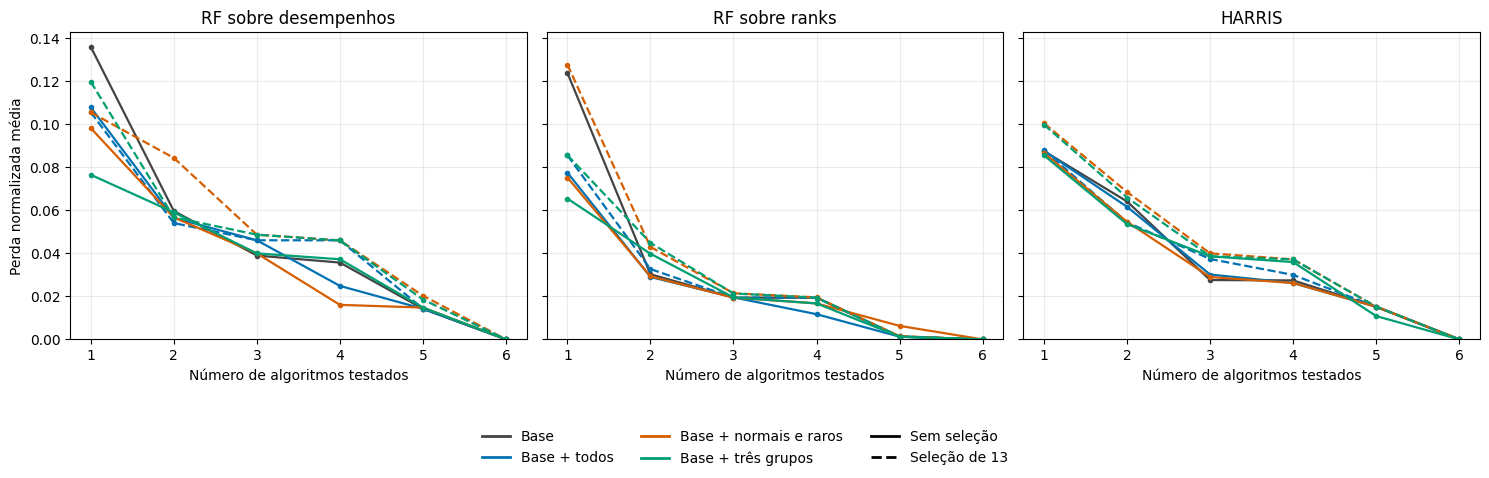
\includegraphics[width=0.70\textwidth]{figuras/curvas_perda_representacoes.png}\\[-2pt]
{\small Perda média ao testar os $t$ primeiros regressores recomendados. Linhas tracejadas: com seleção de 13 atributos.}
\end{figure}

Nas médias, as novas medidas melhoraram as duas abordagens com Random Forest. Na Abordagem 2, a área caiu de 0,032 para 0,023 com as medidas do conjunto completo (cerca de 28\% a menos), e o maior Spearman (0,558) foi obtido com normais e raros. Juntar os três grupos (51 atributos) não superou as extensões menores, e o HARRIS não teve melhora consistente. A seleção de 13 atributos piorou a área em todas as nove combinações.

Para verificar se essas diferenças vão além do acaso, comparamos as sete configurações de cada abordagem (original, três extensões e as mesmas três com seleção) com o teste de Friedman sobre as áreas dos 30 datasets, seguido do teste de Nemenyi. O nível de significância foi dividido entre as três abordagens (0,05/3).

\begin{center}
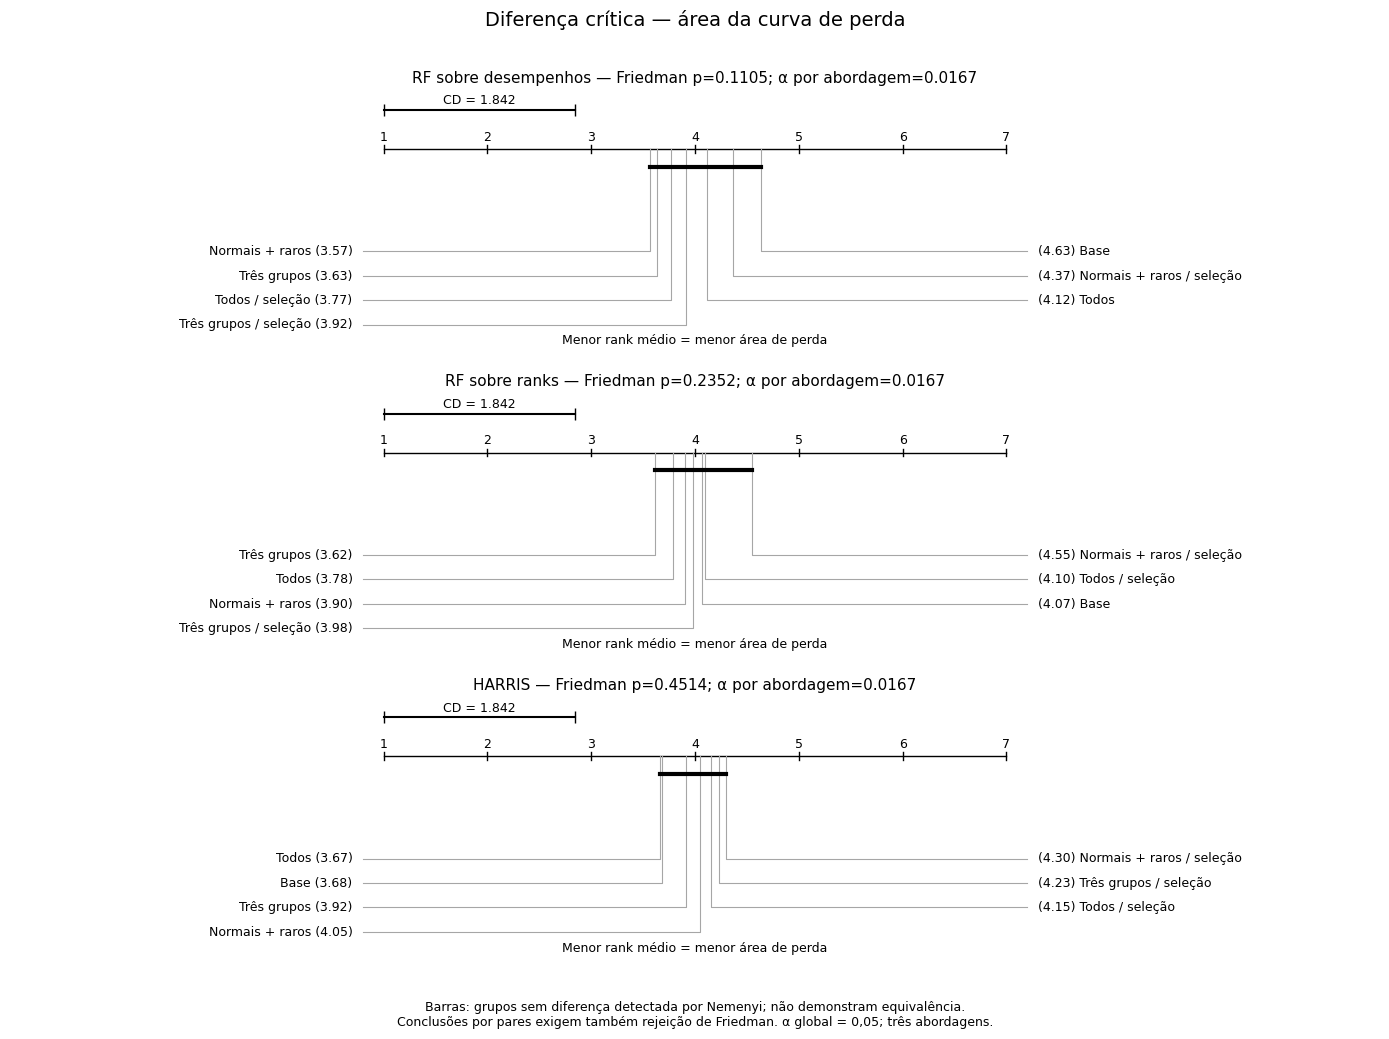
\includegraphics[width=0.80\textwidth]{figuras/diferenca_critica_area.png}

\small
\begin{tabular}{lr}
\toprule
Abordagem & $p$ (Friedman) \\
\midrule
1 (RF sobre desempenhos) & 0,11 \\
2 (RF sobre ranks) & 0,24 \\
HARRIS & 0,45 \\
\bottomrule
\end{tabular}

{\footnotesize Nenhum $p$ ficou abaixo de 0,0167. No diagrama, menor rank médio é melhor, e configurações ligadas por uma barra não diferem significativamente.}
\end{center}

O teste não encontrou diferença significativa em nenhuma abordagem: as sete configurações ficaram dentro da mesma diferença crítica (1,84). As melhoras observadas nas médias, portanto, não se sustentam estatisticamente.

\section{Interpretação e conclusão}

Separar normais e raros mostrou aspectos que a proporção de raros não revela. A região mais difícil muda de um dataset para outro, e as novas medidas mais associadas ao rank de KNN, regressão linear e RF são justamente as dos raros. Já as medidas do conjunto completo e as dos normais se sobrepõem bastante.

Quanto à recomendação, houve melhora nas médias das abordagens com Random Forest, mas, estatisticamente, o sistema ficou igual. Atribuímos esse resultado sobretudo ao tamanho do meta-dataset: são até 51 atributos, com 34 pares redundantes, para 29 datasets de treino por rodada. O sinal também é fraco, pois nenhuma medida passa de 0,45 de correlação com o rank, e a mais útil muda conforme o regressor. Além disso, a margem para melhorar é pequena: o rank médio, que nem usa as meta-características, já chega a Spearman 0,544 e área 0,027, perto do melhor resultado obtido (0,023). A seleção de atributos não resolveu o excesso de colunas, provavelmente porque escolhe as medidas pela associação média com os seis ranks, enquanto cada regressor depende de medidas diferentes.

Sem ganho comprovado, os 31 minutos de extração não se justificam nesta tarefa. Como C3 ocupa 97\% desse tempo e é muito correlacionada com C1 ($-0{,}96$), o passo natural é repetir a avaliação sem ela, o que reduziria o custo para menos de um minuto.

Os resultados têm limitações. As associações com o rank são exploratórias, sem teste de significância, e há mais medidas novas que originais, o que aumenta a chance de surgirem valores altos entre elas. O rank mede desempenho relativo, e não erro absoluto. Os tempos valem para a sessão do Colab utilizada. Por fim, a ausência de diferença significativa não prova que as representações sejam equivalentes: com 30 datasets, o teste só detectaria diferenças grandes.

Para a pesquisa em seleção dinâmica de modelos para regressão desbalanceada, que avalia a competência dos modelos em regiões locais dos dados, fica a indicação de que quantidade de raros, variação local e dificuldade de previsão são propriedades distintas. As medidas por grupo descrevem bem os dados, mas, para usá-las na previsão de desempenho, será preciso reunir mais datasets ou reduzir o número de colunas.

\section{Próximos passos}

Algumas análises ficaram pendentes. A mais direta é repetir a avaliação sem C3, para saber se ela contribui ou pode ser descartada. Também pretendemos reduzir a redundância antes de selecionar atributos, mantendo uma medida de cada grupo de medidas muito correlacionadas, e testar uma seleção feita por regressor, em vez da média dos seis ranks. Outra possibilidade é calcular as medidas separadamente para os raros das caudas alta e baixa, que hoje formam um único grupo. Por fim, vale verificar a robustez dos resultados variando o limiar de relevância e a semente do Random Forest, e ampliar a base com mais datasets de regressão desbalanceada.

\begingroup
\footnotesize
\begin{thebibliography}{9}
\setlength{\itemsep}{0pt}
\bibitem{lorena} Lorena, A. C. et al. (2018). Data complexity meta-features for regression problems. \emph{Machine Learning}, 107, 209--246. \href{https://doi.org/10.1007/s10994-017-5681-1}{doi:10.1007/s10994-017-5681-1}.
\bibitem{avelino} Avelino, J. G.; Cavalcanti, G. D. C.; Cruz, R. M. O. (2025). Imbalanced regression pipeline recommendation. \emph{Machine Learning}, 114, 146. \href{https://doi.org/10.1007/s10994-025-06766-5}{doi:10.1007/s10994-025-06766-5}.
\bibitem{ribeiro} Ribeiro, R. P.; Moniz, N. (2020). Imbalanced regression and extreme value prediction. \emph{Machine Learning}, 109, 1803--1835. \href{https://doi.org/10.1007/s10994-020-05900-9}{doi:10.1007/s10994-020-05900-9}.
\end{thebibliography}
\endgroup

\clearpage
\appendix
\section{Tabela do levantamento}

Todas as medidas pertencem à família de complexidade da taxonomia vista em aula e foram propostas por Lorena et al.\ \cite{lorena}, com exceção de S1\_sd, uma agregação complementar de S1 considerada no levantamento do Meta-IR \cite{avelino}. Há implementações disponíveis em \href{https://github.com/aclorena/ComplexityRegression}{ComplexityRegression} (R) e na biblioteca \href{https://github.com/lpfgarcia/ECoL}{ECoL}; usamos implementações próprias em Python, no notebook, com as adaptações indicadas. A contribuição específica para o domínio é o cálculo nos três grupos definidos pela relevância. O custo é o tempo total nas 90 combinações de dataset e grupo; medidas calculadas juntas aparecem com o mesmo tempo.

\begin{center}
\footnotesize
\renewcommand{\arraystretch}{1.2}
\begin{tabularx}{\textwidth}{@{}p{1.0cm}YY>{\raggedright\arraybackslash}p{1.6cm}Y@{}}
\toprule
Medida & O que se calcula & O que captura no problema & Custo (s) & Situação \\
\midrule
\multicolumn{5}{@{}l}{\textit{Correlação}} \\
C1 & Maior correlação de Spearman (em módulo) entre um preditor e o alvo & Se algum preditor, sozinho, acompanha o alvo no grupo & 2,3 (C1+C2) & Extraída; preditores constantes excluídos \\
C2 & Média dessas correlações & Se a associação está espalhada entre os preditores & 2,3 (C1+C2) & Extraída \\
C3 & Menor fração de exemplos a remover para um preditor atingir correlação 0,9 & Quantos exemplos discordam da ordem do alvo, por exemplo raros fora do padrão & 1.807,1 & Extraída; nove valores ausentes \\
C4 & Fração de exemplos que sobra após ajustes lineares sucessivos, um preditor por vez & Quanto do grupo os preditores conseguem explicar em conjunto & 8,6 & Extraída; cada preditor usado uma vez \\
\midrule
\multicolumn{5}{@{}l}{\textit{Linearidade}} \\
L1 & Erro absoluto médio de uma regressão linear & Se o grupo segue uma relação linear & 1,4 (L1+L2) & Extraída; quatro ajustes saturados \\
L2 & Erro quadrático médio da mesma regressão & Idem, dando mais peso a erros grandes & 1,4 (L1+L2) & Extraída \\
L3 & Erro da regressão em pontos interpolados entre exemplos vizinhos & Se a relação linear vale também entre os exemplos & 0,6 & Extraída \\
\midrule
\multicolumn{5}{@{}l}{\textit{Suavidade}} \\
S1 & Diferença média do alvo entre exemplos ligados na árvore geradora mínima & Variação local do alvo: se vizinhos têm alvos próximos & 18,2 (S1+S1\_sd) & Extraída \\
S1\_sd & Desvio-padrão dessas diferenças & Se a variação local é homogênea ou concentrada & 18,2 (S1+S1\_sd) & Extraída \\
S2 & Distância média entre exemplos consecutivos na ordem do alvo & Se alvos próximos correspondem a preditores próximos & 0,2 (S2+T2) & Extraída \\
S3 & Erro de prever cada exemplo pelo vizinho mais próximo & Previsibilidade local, que pode ser pior na região rara & 13,9 & Extraída \\
S4 & Erro do vizinho mais próximo em pontos interpolados & Complementa S3 entre os exemplos & 9,7 & Extraída \\
\midrule
\multicolumn{5}{@{}l}{\textit{Dimensionalidade}} \\
T2 & Número de exemplos por preditor & Quantos dados sustentam cada grupo & 0,2 (S2+T2) & Global retirada, por repetir a referência \\
\bottomrule
\end{tabularx}
\end{center}

Nenhuma medida planejada ficou de fora por falta de implementação, custo ou incompatibilidade com os dados. Os nove valores ausentes de C3 vêm de uma regra conservadora: quando a correlação ficava indefinida antes do limiar, o valor não foi registrado. Os quatro ajustes lineares saturados (os três grupos de \texttt{pdgfr} e os raros de \texttt{cocomo\_numeric}) pedem cautela na leitura de L1--L3 nesses casos.

\end{document}
